\documentclass[a4paper]{article}

\usepackage[hidelinks]{hyperref}
\usepackage[notquote]{hanging}
\usepackage{siunitx}
\usepackage{amsmath}
\usepackage[margin=1in]{geometry}
\usepackage{pgfplots}
\pgfplotsset{width=10cm, compat=newest}
\usepackage{setspace}
\usepackage{minted}

\begin{document}
\title{The Relationship Between The Amount of Sodium Chloride in a Sodium
Chloride Solution and Oxygen Saturation of the solution}
\author{Marko Vejnovi\'{c}}

\maketitle

\doublespacing

\section*{Rationale}

\paragraph*{}
Regarding chemistry overall, I am most interested in industrial chemistry. Due
to my affinity for physics and engineering, I am naturally drawn to everything
regarding engineering, including industrial chemistry. My original idea for my
internal assessment was to conduct experiments which would show show the
relationship between the voltage applied and the thickness of the anodized
layer in a process of aluminum anodization. However, as preliminary
experiments showed, the thickness of this layer was immeasurable with the tools
available.

\paragraph*{}
I, therefore decided to apply another passion of mine, one which sadly I was
not able to pursue in my last two years of high school education -
environmental chemistry. Being always passionate for biology and ecology, I
decided to look into phenomena that govern the sustainability and longevity of
biotopes\footnote{Regions of homogeneous environmental conditions and
populations of organisms (Merriam Webster)}. Being a diver, it was clear to me
that I wanted to do research to see how chemistry could be applied in aqueous
environmental systems. Knowing that oxygen saturation is a major factor in the
habitability of aqueous biotopes, I knew that I wanted to measure the
relationship between the salinity of water and the oxygen saturation in it.

\section{Introduction}

\subsection{Oxygen saturation}

\paragraph*{}
Oxygen saturation\footnote{Synonymous with dissolved oxygen} is the measure of
of the amount of oxygen dissolved in water measured in $\left[
\frac{\si{g}}{\si{l}} \right]$ (Utah State University Extension).

\paragraph*{}
As all aerobic organisms require oxygen, aquatic lifeforms all require a
sufficient amount of dissolved oxygen. However, an over-abundance in dissolved
oxygen can, although it is unlikely, induce the \textit{gas bubble disease},
which cause hyperinflation of all fish organs which contain air.

\paragraph*{}
The process through which oxygen dissolves into water is usually due to a
pressure difference between the partial pressure of oxygen in the atmosphere
and the pressure of oxygen in water.

\paragraph*{}
Oxygen becomes ``stuck'' in between water molecules which are bounded by
hydrogen bonds (Senese). A figure representing this mechanism is given in
figure \ref{fig:do}.

\begin{figure}[ht]
  \centering
  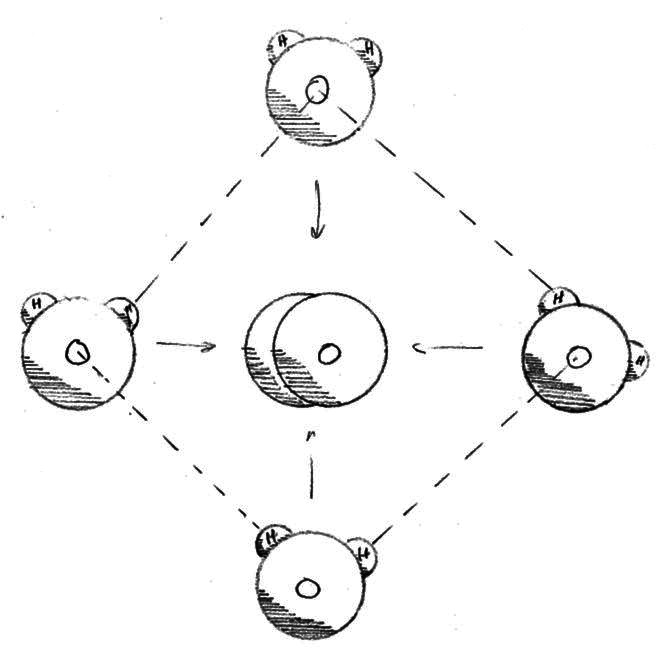
\includegraphics[width=0.5\textwidth]{img/do}
  \caption{How oxygen dissolves in water}
  \label{fig:do}
\end{figure}

\subsection{Salinity}

\paragraph*{}
Salinity is the measure of dissolved salts in water, measured in either $\left[
\frac{\si{g}}{\si{l}} \right]$ or $\left[ \frac{g}{kg} \right]$ (``Key Physical
Variables In The Ocean: Temperature, Salinity, And Density''). Due to the fact
that all of the salts in water are predominantly are $NaCl$ molecules, the term
salinity onward in this paper refers to the amount of dissolved $NaCl$
molecules.

\paragraph*{}
Salinity, too, affects the habitability of aqueous habitats, as certain
organisms require salt, yet others can only sustain life in relatively
salt-less bodies of water.

\subsection{Relation between salinity and dissolved oxygen}

\paragraph*{}
The key reason why it is expected of an increase in salinity of water to be
followed by a decrease in the amount of dissolved oxygen is governed by the
fact that water is a polar molecule. As a salt dissolves in water, the polar
salt attracts the water molecules, decreasing the strength of the hydrogen
bonds between water - making it so that the hydrogen bonds between water
molecules cannot keep the oxygen molecules in place as much.

\subsection{Research goal}

\paragraph*{}
The goal of this research is to empirically determine the relationship between
the salinity of water and the maximum dissolved oxygen capacity of water.

\section{Method}

\paragraph*{}
To determine the relationship between the salinity of water and the amount of
dissolved oxygen it was decided that the \textit{Winkler method} would be
employed, due to its relative ease of conduction as well as the availability of
the materials required.

\subsection{Winkler method}

\paragraph*{}
The Winkler method is a chemical process which is used to measure the amount of
dissolved oxygen in water. Normally, it involves four distinct steps.

\paragraph*{}
The first step is adding manganese(II) sulfate, with which oxygen molecules
react under alkaline conditions:
$$2 Mn^{2+}_{(aq)} + O_{2(aq)} + H_2O_{(l)} \rightarrow MnO(OH)_{2(s)}$$
This step allows for binding the oxygen in the water, creating manganese(IV)
ions.

\paragraph*{}
Next, sulfuric acid is added, forming manganese(IV) sulfate:
$$MnO(OH)_{2(s)} + 4H^+_{(aq)} \rightarrow Mn^{4+}_{(aq)} + 3H_2O_{(l)}$$

\paragraph*{}
Sodium(I) iodide is added. Iodide ions become oxidized to $I_2$, creating a
very orange solution.
$$Mn^{4+}_{(aq)} + 2I^-_{(aq)} \rightarrow Mn^{2+}_{(aq)} + I_{2(aq)}$$

\paragraph*{}
The final step involves titrating the iodine against sodium thiosulfate:
$$I_{2(aq)} + 2S_2O_{3(aq)}^{2-} \rightarrow S_4O_{6(aq)}^{2-} + 2I_{(aq)}^-$$

\paragraph*{}
The importance of the method lies in the fact that there is a linear
relationship between the number of moles of thiosulfate used and the number of
moles of oxygen, and that relation is:
$$n(O_2) = \frac{1}{4} n(Na_2S_2O_3)$$

\subsection{Safety and environmental precautions}

\paragraph*{}
The experiment itself was not necessarily dangerous, however, the chemicals
employed were handled with care.

\subsubsection{Manganese(II) sulfate}

\paragraph*{}
Manganese(II) sulfate is dangerous to the environment, so it was disposed of
according to the mentor's requests.

\subsubsection{Sodium Iodide}

\paragraph*{}
Sodium Iodide is both toxic and irritation inducing (``Sodium Iodide''),
therefore, it was handled with the use of safety goggles and latex gloves. Due
to it being extremely toxic to aquatic life, it was disposed of in accordance
with the mentor's advice.

\subsubsection{Sodium thiosulfate}

\paragraph*{}
Sodium thiosulfate induces skin irritations (``Sodium Thiosulfate''), so it was
handled with care. 

\subsubsection{Sulfuric acid}

\paragraph*{}
Sulfuric acid is highly irritating and causes permanent eye damage (``Sulfuric
Acid''). Because of this, eye goggles were worn at all times. Due to its very
high acidic properties, a base ($NaOH$) was present nearby to neutralize any
potential spills that might occur. Incidentally, a minor spill did occur, and
the basic sodium hydroxide was used to neutralize the acid, after which it was
cleaned up with water.

\paragraph*{}
After the experiment, the remaining sulfuric acid was disposed of per
school protocol - in a separate container for acidic solutions.

\subsection{Method}

\subsubsection{Solutions}

\paragraph*{}
Before the actual experiment could be conducted, some solutions had to be
prepared.

\paragraph*{Sodium iodide}
A Sodium iodide solution was prepared by adding sodium iodide to a solution of
sodium hydroxide. The exact concentration of this solution is not important, as
long as it is assured that sodium iodide is in excess.

\paragraph*{Starch solution}
A solution of starch to be used as an indicator was done by dissolving starch
in distilled water under light temperature and with mild stirring. The
concentration is again irrelevant.

\paragraph*{Sodium thiosulfate}
A sodium thiosulfate solution was prepared by dissolving sodium thiosulfate in
distilled water.

\begin{figure}[ht]
  \centering
  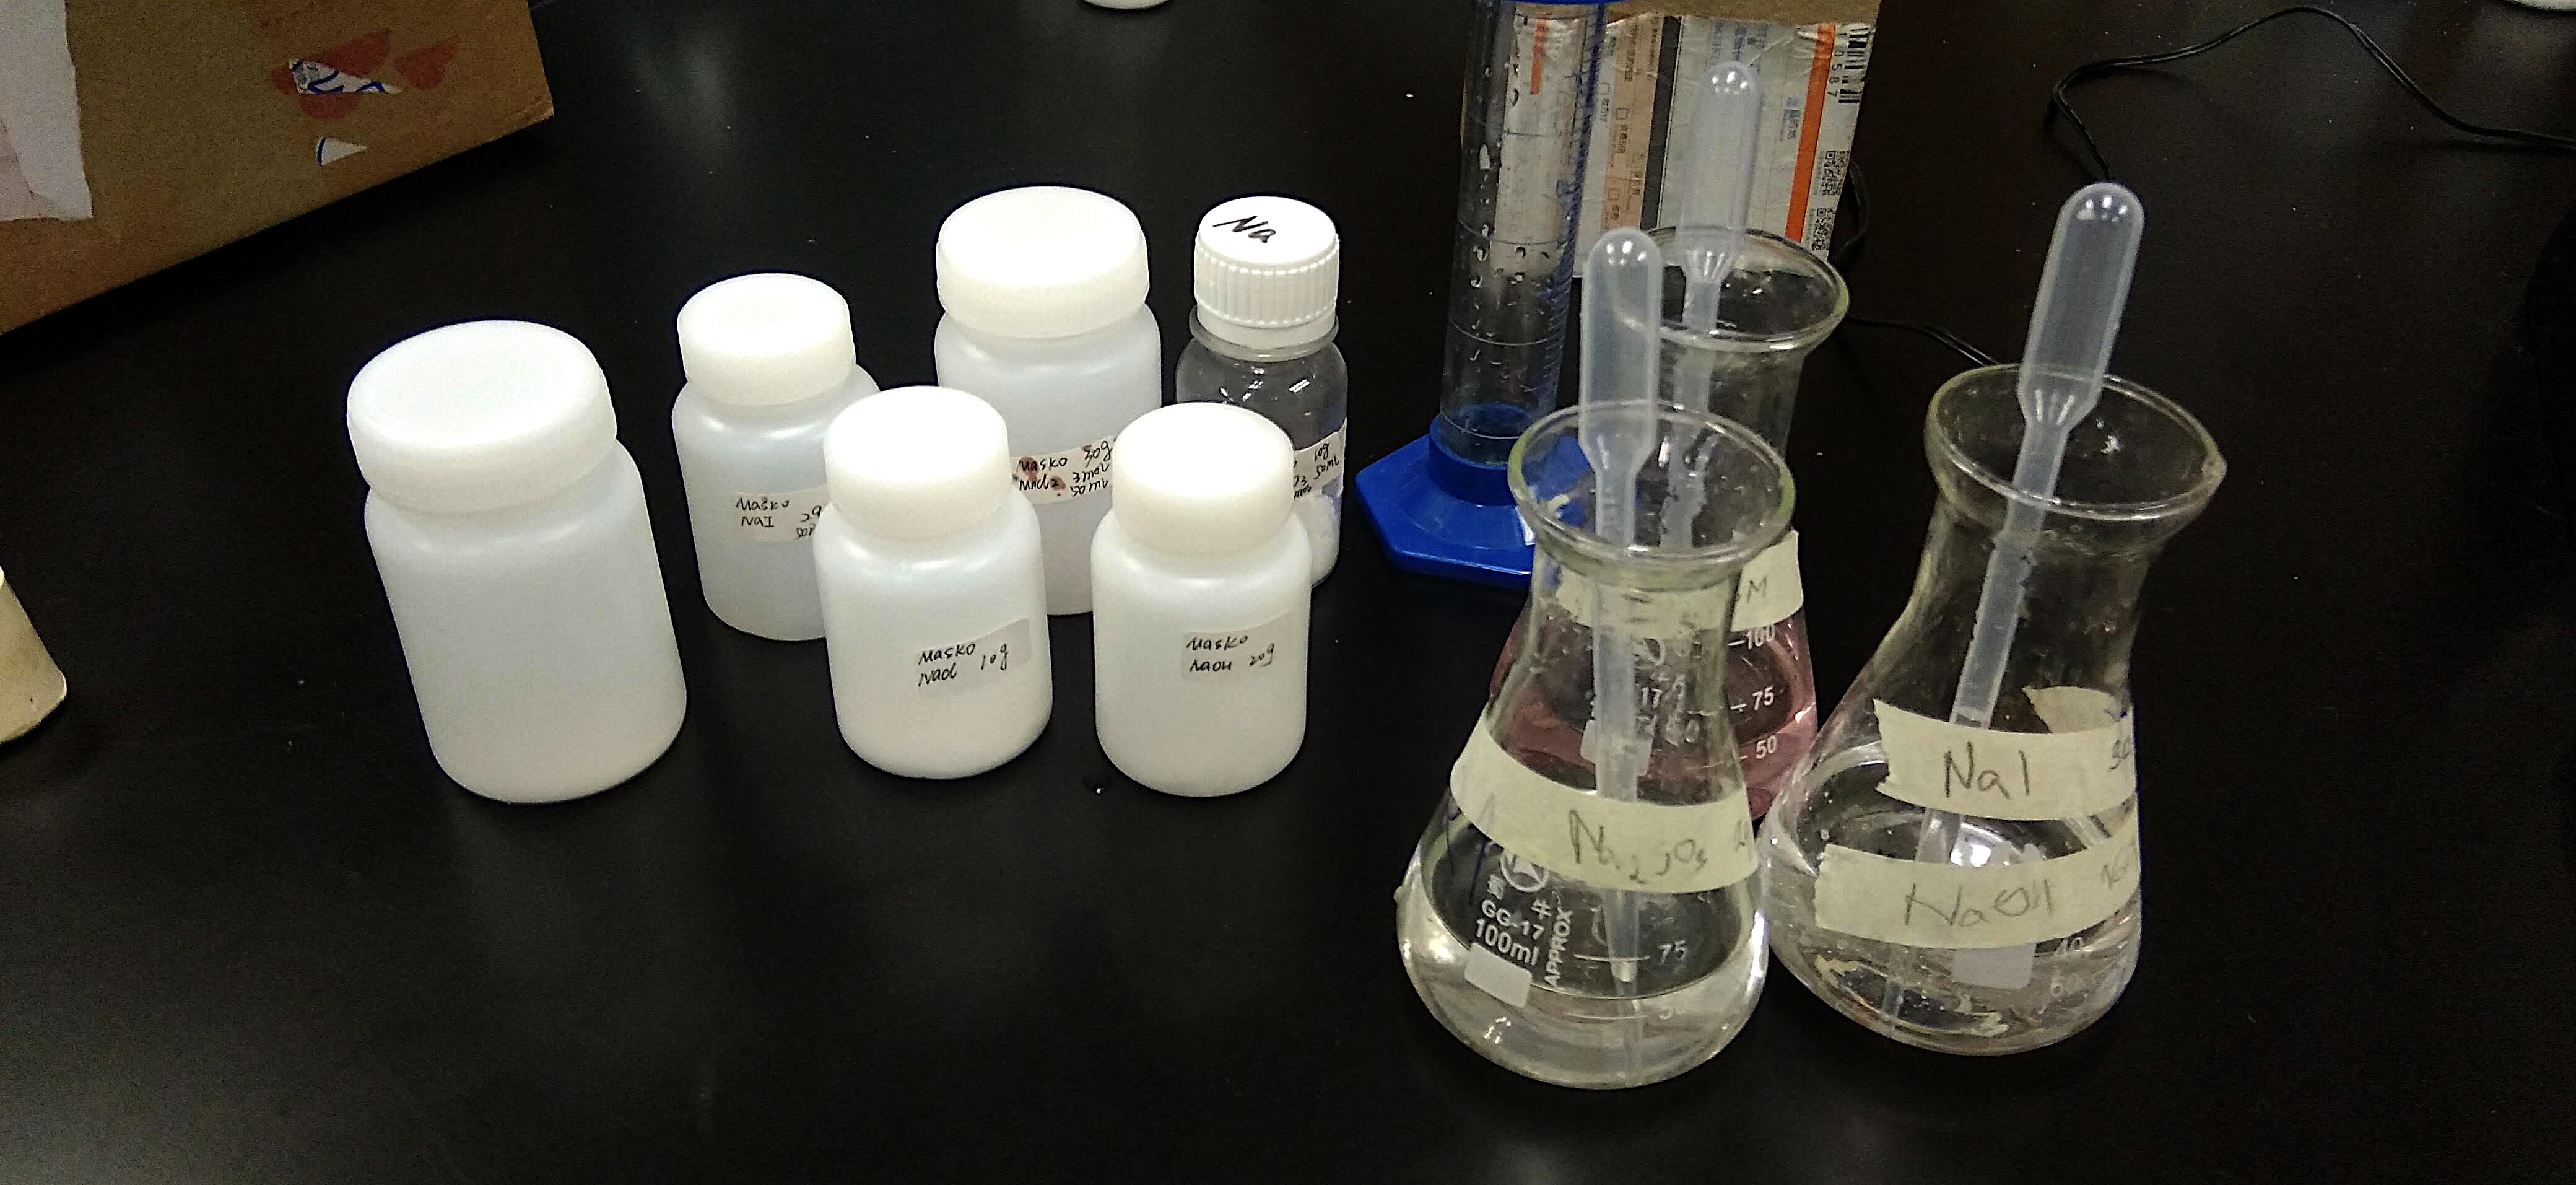
\includegraphics[width=0.5\textwidth]{img/solutions}
  \caption{The prepared solutions}
\end{figure}

\paragraph*{Saline solutions}
The $NaCl$ solutions were not prepared prior to the experiment as doing that
would make the times between adding the salt and titrating the solution.
However, a $100\si{ml}$ of distilled water was poured in plastic containers in
which the titration would be done.

\subsubsection{Experiment}

\paragraph*{}
With the solutions prepared it was possible to conduct the experiment.
Throughout the whole experiment the temperature was kept a constant:
$$t = 20\si{\degree C}$$
It was assumed that pressure was constant.

\paragraph*{}
First, water was poured into $6$ plastic containers of $100\si{ml}$. Plastic
containers were used because of the fact that they are closable, unlike
beakers.

\paragraph*{}
Next, $NaCl$ was dissolved in each of these containers. Given that the maximal
solubility of $NaCl$ in water is $\frac{36\si{g}}{100\si{ml}}$ (Rumble, John
R.), it was decided that the salt would be added in increments of $6\si{g}$.
The maximum salt mass for this value is $30 \si{g}$. The choice of making the
maximum $30\si{g}$ rather than $36\si{g}$ was made due to two reasons - one
being that it was easily possible that some salt would not dissolve due to
errors when measuring the volume of water and the mass of the salt - and the
other, more important one being that when a relationship is established, it
should be able to predict a minimum of oxygen dissolved at around $36\si{g}$.

\paragraph*{}
Since this experiment requires a constant amount of oxygen to be dissolved in
water, and since the maximum saturation of oxygen is being tested for, it was
decided that a magnetic stirrer would be used at maximum power to increase the
amount of oxygen dissolved in water to its maximal capacity. It was made sure
that the power of the magnetic was not too high to be able to form bubbles
inside the container. To make sure that this amount was constant between all
trials, the time of the ``oxidization'' of water was kept constant at $1$
minute between all trials.

\paragraph*{}
After each bottle was saturated with oxygen, manganese(II) sulfate was added to
the bottle using a plastic pipette. This process was repeated until
manganese(II) sulfate was added to all bottles.

\paragraph*{}
The first bottle was placed on a magnetic stirrer which was set to lightly
stir, but remained turned off. A burette containing sodium thiosulfate was
placed over the stirrer. Sulfuric acid was added to the bottle and the stirrer
was powered on. Titration was done until the solution reached an extremely pale
yellow color at which point starch was added, as shown in figure
\ref{fig:titration}. This caused the solution to become blue. It was then
titrated to the point of the solution becoming translucent.

\begin{figure}[ht]
  \centering
  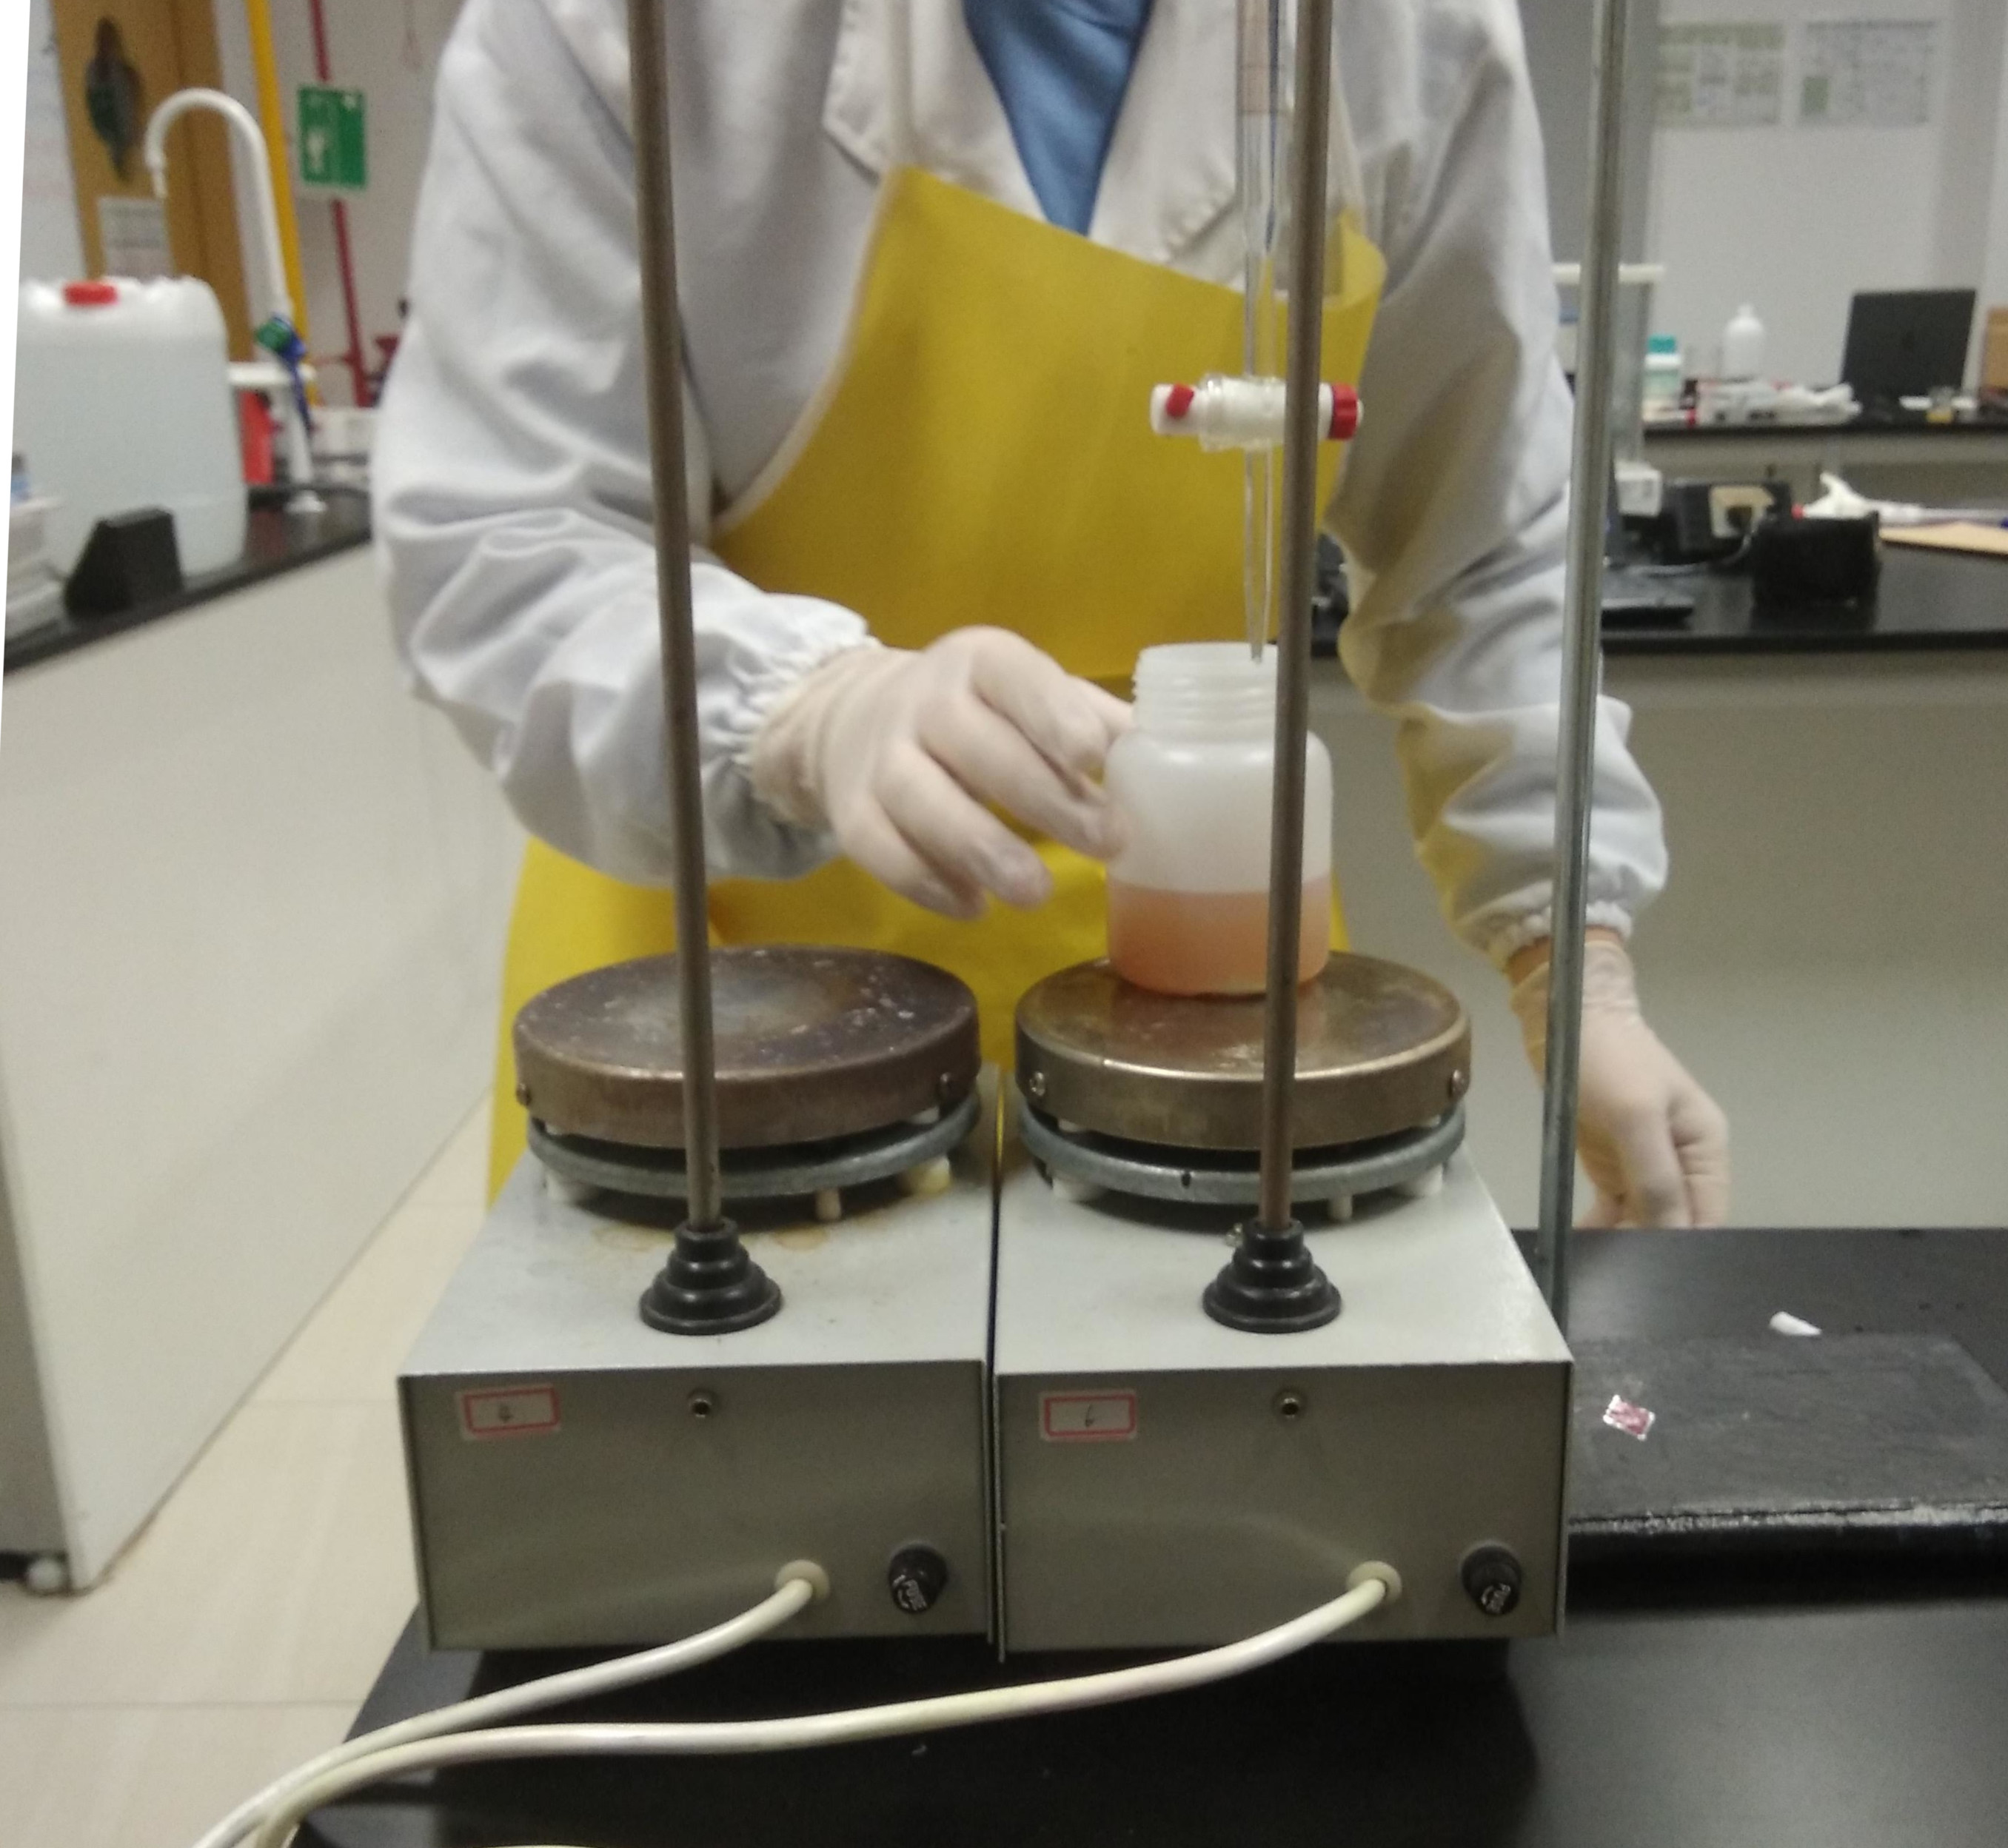
\includegraphics[width=0.6\textwidth]{img/titration}
  \caption{Titration}
  \label{fig:titration}
\end{figure}

\section{Data}

\subsection{Raw Data}

\paragraph*{}
The raw data is presented in the following.

\subsubsection{Manganese(II) sulfate solution}

\paragraph*{}
The concentration of the solution was:
$$c(MnSO_4) = 3\si{M}$$

\subsubsection{Sodium Iodide solution}

\paragraph*{}
The volume of the water in the solution was:
$$V(H_2O) = (50.0 \pm 0.5) \si{ml}$$

\paragraph*{}
The mass of the solutes was:
$$m(NaI) = (30.00 \pm 0.01) \si{g}$$
$$m(NaOH) = (16 \pm 0.01) \si{g}$$

\subsubsection{Sulfuric acid}

\paragraph*{}
The concentrated sulfuric acid was $50\%$ by volume.

\subsubsection{Starch solution}

\paragraph*{}
The volume of water was:
$$V(H_2O) = (50 \pm 0.5) \si{ml}$$

\paragraph*{}
The mass of the solute starch was:
$$m\left( \left( C_6 H_{10} O_5 \right)_n \right) = (2.00 \pm 0.01) \si{g}$$

\subsubsection{Sodium thiosulfate solution}

\paragraph*{}
The volume of water was:
$$V(H_2O) = (50.0 \pm 0.5) \si{ml}$$

\paragraph*{}
The mass of sodium thiosulfate was:
$$m(Na_2SO_3) = (2.00 \pm 0.01) \si{g}$$

\subsubsection{Titration}

\paragraph*{}
The measurements obtained during the titrations are given in the tables
\ref{tbl:titration-1}, \ref{tbl:titration-2} and \ref{tbl:titration-3}.

\begin{table}[ht]
  \center
  \begin{tabular}{r | r | r | r | r }
    \# & $V(H_2O)$ & $m(NaCl)$ & Starting $V(Na2SO_3)$ & Ending $V(Na_2SO_3)$
    \\ \hline \hline
    1 & $(100.0 \pm 0.5) \si{ml}$ & $0 \si{g}$ & $(16.90 \pm 0.05) \si{ml}$ &
    $(17.9 \pm 0.05) \si{ml}$ \\ \hline
    2 & $(100.0 \pm 0.5) \si{ml}$ & $(6.03 \pm 0.01) \si{g}$ & $(17.90 \pm
    0.05) \si{ml}$ & $(18.70 \pm 0.05) \si{ml}$ \\ \hline
    3 & $(100.0 \pm 0.5) \si{ml}$ & $(12.03 \pm 0.01) \si{g}$ & $(18.70 \pm
    0.05) \si{ml}$ & $(19.40 \pm 0.05) \si{ml}$ \\ \hline
    4 & $(100.0 \pm 0.5) \si{ml}$ & $(18.01 \pm 0.01) \si{g}$ & $(19.40 \pm
    0.05) \si{ml}$ & $(20.00 \pm 0.05) \si{ml}$ \\ \hline
    5 & $(100.0 \pm 0.5) \si{ml}$ & $(23.95 \pm 0.01) \si{g}$ & $(20.00 \pm
    0.05) \si{ml}$ & $(20.40 \pm 0.05) \si{ml}$ \\ \hline
    6 & $(100.0 \pm 0.5) \si{ml}$ & $(30.03 \pm 0.01) \si{g}$ & $(20.40 \pm
    0.05) \si{ml}$ & $(20.90 \pm 0.05) \si{ml}$ \\ \hline
  \end{tabular}
  \caption{The measurements obtained during the first titration
  \label{tbl:titration-1}}
\end{table}

\begin{table}[ht]
  \center
  \begin{tabular}{r | r | r | r | r }
    \# & $V(H_2O)$ & $m(NaCl)$ & Starting $V(Na2SO_3)$ & Ending $V(Na_2SO_3)$
    \\ \hline \hline
    1 & $(100.0 \pm 0.5) \si{ml}$ & $0 \si{g}$ & $(20.90 \pm 0.05) \si{ml}$ &
    $(21.80 \pm 0.05) \si{ml}$ \\ \hline
    2 & $(100.0 \pm 0.5) \si{ml}$ & $(6.07 \pm 0.01) \si{g}$ & $(21.80 \pm
    0.05) \si{ml}$ & $(22.50 \pm 0.05) \si{ml}$ \\ \hline
    3 & $(100.0 \pm 0.5) \si{ml}$ & $(12.01 \pm 0.01) \si{g}$ & $(22.50 \pm
    0.05) \si{ml}$ & $(23.10 \pm 0.05) \si{ml}$ \\ \hline
    4 & $(100.0 \pm 0.5) \si{ml}$ & $(17.99 \pm 0.01) \si{g}$ & $(23.10 \pm
    0.05) \si{ml}$ & $(23.60 \pm 0.05) \si{ml}$ \\ \hline
    5 & $(100.0 \pm 0.5) \si{ml}$ & $(24.01 \pm 0.01) \si{g}$ & $(23.60 \pm
    0.05) \si{ml}$ & $(24.10 \pm 0.05) \si{ml}$ \\ \hline
    6 & $(100.0 \pm 0.5) \si{ml}$ & $(30.00 \pm 0.01) \si{g}$ & $(24.10 \pm
    0.05) \si{ml}$ & $(24.50 \pm 0.05) \si{ml}$ \\ \hline
  \end{tabular}
  \caption{The measurements obtained during the second titration
  \label{tbl:titration-2}}
\end{table}

\begin{table}[ht]
  \center
  \begin{tabular}{r | r | r | r | r }
    \# & $V(H_2O)$ & $m(NaCl)$ & Starting $V(Na2SO_3)$ & Ending $V(Na_2SO_3)$
    \\ \hline \hline
    1 & $(100.0 \pm 0.5) \si{ml}$ & $0 \si{g}$ & $(24.50 \pm 0.05) \si{ml}$ &
    $(25.40 \pm 0.05) \si{ml}$ \\ \hline
    2 & $(100.0 \pm 0.5) \si{ml}$ & $(6.04 \pm 0.01) \si{g}$ & $(25.40 \pm
    0.05) \si{ml}$ & $(26.10 \pm 0.05) \si{ml}$ \\ \hline
    3 & $(100.0 \pm 0.5) \si{ml}$ & $(11.58 \pm 0.01) \si{g}$ & $(26.10 \pm
    0.05) \si{ml}$ & $(26.70 \pm 0.05) \si{ml}$ \\ \hline
    4 & $(100.0 \pm 0.5) \si{ml}$ & $(18.03 \pm 0.01) \si{g}$ & $(26.70 \pm
    0.05) \si{ml}$ & $(27.30 \pm 0.05) \si{ml}$ \\ \hline
    5 & $(100.0 \pm 0.5) \si{ml}$ & $(24.02 \pm 0.01) \si{g}$ & $(27.30 \pm
    0.05) \si{ml}$ & $(27.80 \pm 0.05) \si{ml}$ \\ \hline
    6 & $(100.0 \pm 0.5) \si{ml}$ & $(29.99 \pm 0.01) \si{g}$ & $(27.80 \pm
    0.05) \si{ml}$ & $(28.20 \pm 0.05) \si{ml}$ \\ \hline
  \end{tabular}
  \caption{The measurements obtained during the third titration
  \label{tbl:titration-3}}
\end{table}

\subsection{Data Processing}

\subsubsection{Sodium Iodide solution}

\paragraph*{}
The concentration of the sodium iodide solution was equal to:
\begin{align*}
  c(NaI) 
  &= \frac{n(NaI)}{V(H_2O)} \\
  &= \cfrac{\cfrac{(30.00 \pm 0.01)\si{g}}{149.89\si{\frac{g}{mol}}}}{(50.0 \pm
    0.5) \cdot 10^{-3} \si{l}} \\
  c(NaI) &= (4.00 \pm 0.04) \si{M}
\end{align*}

\subsubsection{Starch solution}

\paragraph*{}
Due to the fact that starch is a polymer of glucose monomers, it was impossible
to accurately calculate the concentration of the starch indicator solution,
however, this piece of information was irrelevant, since starch was only acting
as an indicator.

\subsubsection{Sodium thiosulfate solution}

\paragraph*{}
The concentration of the sodium thiosulfate solution was:
\begin{align*}
  c(Na_2SO_3) 
  &= \frac{n(Na_2SO_3)}{V(H_2O)} \\
  &= \cfrac{\cfrac{(2.00 \pm 0.01)\si{g}}{126.05\si{\frac{g}{mol}}}}{(50.0 \pm
    0.5) \cdot 10^{-3} \si{l}} \\
  c(Na_2SO_3) &= (0.317 \pm 0.005) \si{M}
\end{align*}

\subsubsection{Titration}

\paragraph*{}
The amount of sodium thiosulfate used was calculated by subtracting the ending
volumes and starting volumes of sodium thiosulfate in the burette. The results
are given in tables \ref{tbl:calc-titration-1}, \ref{tbl:calc-titration-2} and
\ref{tbl:calc-titration-3}.

\begin{table}[ht]
  \center
  \begin{tabular}{ r | r | r | r }
    \# & $V(H_2O) \left[ \pm 0.5 \si{ml} \right]$ & $m(NaCl) \left[ \pm 0.01
      \si{g} \right]$ & $\Delta V(Na2SO_3) \left[ \pm 0.10 \si{ml} \right]$ \\
      \hline \hline
    1 & $100.0 \si{ml}$ & $0.00 \si{g}$ & $1.00 \si{ml}$ \\ \hline
    2 & $100.0 \si{ml}$ & $6.03 \si{g}$ & $0.80 \si{ml}$ \\ \hline
    3 & $100.0 \si{ml}$ & $12.03 \si{g}$ & $0.70 \si{ml}$ \\ \hline
    4 & $100.0 \si{ml}$ & $18.01 \si{g}$ & $0.60 \si{ml}$ \\ \hline
    5 & $100.0 \si{ml}$ & $23.95 \si{g}$ & $0.40 \si{ml}$ \\ \hline
    6 & $100.0 \si{ml}$ & $30.03 \si{g}$ & $0.50 \si{ml}$ \\ \hline
  \end{tabular}
  \caption{The mass of salt vs. the volume of sodium thiosulfate used in the
    first titration \label{tbl:calc-titration-1}}
\end{table}

\begin{table}[ht]
  \center
  \begin{tabular}{ r | r | r | r }
    \# & $V(H_2O) \left[ \pm 0.5 \si{ml} \right]$ & $m(NaCl) \left[ \pm 0.01
      \si{g} \right]$ & $\Delta V(Na2SO_3) \left[ \pm 0.10 \si{ml} \right]$ \\
      \hline \hline
    1 & $100.0 \si{ml}$ & $0.00 \si{g}$ & $0.90 \si{ml}$ \\ \hline
    2 & $100.0 \si{ml}$ & $6.07 \si{g}$ & $0.70 \si{ml}$ \\ \hline
    3 & $100.0 \si{ml}$ & $12.01 \si{g}$ & $0.60 \si{ml}$ \\ \hline
    4 & $100.0 \si{ml}$ & $17.99 \si{g}$ & $0.50 \si{ml}$ \\ \hline
    5 & $100.0 \si{ml}$ & $24.01 \si{g}$ & $0.50 \si{ml}$ \\ \hline
    6 & $100.0 \si{ml}$ & $30.00 \si{g}$ & $0.40 \si{ml}$ \\ \hline
  \end{tabular}
  \caption{The mass of salt vs. the volume of sodium thiosulfate used in the
    second titration \label{tbl:calc-titration-2}}
\end{table}

\begin{table}[ht]
  \center
  \begin{tabular}{ r | r | r | r }
    \# & $V(H_2O) \left[ \pm 0.5 \si{ml} \right]$ & $m(NaCl) \left[ \pm 0.01
      \si{g} \right]$ & $\Delta V(Na2SO_3) \left[ \pm 0.10 \si{ml} \right]$ \\
      \hline \hline
    1 & $100.0 \si{ml}$ & $0.00 \si{g}$ & $0.90 \si{ml}$ \\ \hline
    2 & $100.0 \si{ml}$ & $6.04 \si{g}$ & $0.70 \si{ml}$ \\ \hline
    3 & $100.0 \si{ml}$ & $11.58 \si{g}$ & $0.60 \si{ml}$ \\ \hline
    4 & $100.0 \si{ml}$ & $18.03 \si{g}$ & $0.60 \si{ml}$ \\ \hline
    5 & $100.0 \si{ml}$ & $24.02 \si{g}$ & $0.50 \si{ml}$ \\ \hline
    6 & $100.0 \si{ml}$ & $29.99 \si{g}$ & $0.40 \si{ml}$ \\ \hline
  \end{tabular}
  \caption{The mass of salt vs. the volume of sodium thiosulfate used in the
    third titration \label{tbl:calc-titration-3}}
\end{table}

\paragraph*{}
The average of the data of all three titrations was calculated, as well as the
errors according to the formula $\Delta x = \frac{x_{max} - x_{min}}{2}$. Both
the averages and the uncertainties are given in table
\ref{tbl:calc-titration-final}.
\begin{table}[ht]
  \center
  \begin{tabular}{ r | r | r }
    \# & $\overline{m}(NaCl)$ & $\overline{V}(Na2SO_3)$ \\ \hline \hline
    1 & $0.00 \si{g}$ & $(0.93 \pm 0.15) \si{ml}$ \\ \hline
    2 & $(6.05 \pm 0.03) \si{g}$ & $(0.73 \pm 0.15) \si{ml}$ \\ \hline
    3 & $(11.87 \pm 0.24) \si{g}$ & $(0.63 \pm 0.15) \si{ml}$ \\ \hline
    4 & $(18.01 \pm 0.03) \si{g}$ & $(0.57 \pm 0.15) \si{ml}$ \\ \hline
    5 & $(23.99 \pm 0.05) \si{g}$ & $(0.47 \pm 0.15) \si{ml}$ \\ \hline
    6 & $(30.01 \pm 0.03) \si{g}$ & $(0.43 \pm 0.15) \si{ml}$ \\ \hline
  \end{tabular}
  \caption{The mass of salt vs. the volume of sodium thiosulfate used
  \label{tbl:calc-titration-final}}
\end{table}

\paragraph*{}
Next, the number of moles of sodium thiosulfate used was calculated. The values
are given in table \ref{tbl:calc-na2so3-moles}. This was done according the
following general formula:
$$n(Na2SO_3) = c(Na2SO_3) \cdot V(Na2SO_3)$$
\begin{table}[ht]
  \center
  \begin{tabular}{ r | r | r }
    \# & $\overline{m}(NaCl)$ & $\overline{n}(Na2SO_3)$ \\ \hline \hline
    1 & $0.00 \si{g}$ & $(2.95 \pm 0.52) \cdot 10^{-4} \si{mol}$ \\ \hline
    2 & $(6.05 \pm 0.03) \si{g}$ & $(2.31 \pm 0.51) \cdot 10^{-4} \si{mol}$ \\ \hline
    3 & $(11.87 \pm 0.24) \si{g}$ & $(2.00 \pm 0.51) \cdot 10^{-4} \si{mol}$ \\ \hline
    4 & $(18.01 \pm 0.03) \si{g}$ & $(1.81 \pm 0.50) \cdot 10^{-4} \si{mol}$ \\ \hline
    5 & $(23.99 \pm 0.05) \si{g}$ & $(1.49 \pm 0.50) \cdot 10^{-4} \si{mol}$ \\ \hline
    6 & $(30.01 \pm 0.03) \si{g}$ & $(1.36 \pm 0.50) \cdot 10^{-4} \si{mol}$ \\ \hline
  \end{tabular}
  \caption{The mass of salt vs. the number of moles of sodium thiosulfate used
  \label{tbl:calc-na2so3-moles}}
\end{table}

\paragraph*{}
Finally, the amount of dissolved oxygen was calculated according to the fact
that:
$$DO = \frac{1}{4} n(Na_2SO_3) \cdot 2 \cdot 16.00 \si{\frac{g}{mol}} \cdot
\frac{1}{V(H_2O)}$$
\begin{table}[ht]
  \center
  \begin{tabular}{ r | r | r }
    \# & $\overline{m}(NaCl)$ & $\overline{DO}$ \\ \hline \hline
    1 & $0.00 \si{g}$ & $(2.36 \pm 0.43) \cdot 10^{-2} \si{\frac{g}{l}}$ \\ \hline
    2 & $(6.05 \pm 0.03) \si{g}$ & $(1.85 \pm 0.42) \cdot 10^{-2} \si{\frac{g}{l}}$ \\ \hline
    3 & $(11.87 \pm 0.24) \si{g}$ & $(1.60 \pm 0.42) \cdot 10^{-2} \si{\frac{g}{l}}$ \\ \hline
    4 & $(18.01 \pm 0.03) \si{g}$ & $(1.45 \pm 0.41) \cdot 10^{-2} \si{\frac{g}{l}}$ \\ \hline
    5 & $(23.99 \pm 0.05) \si{g}$ & $(1.19 \pm 0.41) \cdot 10^{-2} \si{\frac{g}{l}}$ \\ \hline
    6 & $(30.01 \pm 0.03) \si{g}$ & $(1.09 \pm 0.41) \cdot 10^{-2} \si{\frac{g}{l}}$ \\ \hline
  \end{tabular}
  \caption{The mass of salt vs. the dissolved oxygen
  \label{tbl:calc-do}}
\end{table}

\section{Analysis}

\subsection{Further calculations} \label{sec:further-calculations}

\paragraph*{}
From table \ref{tbl:calc-do}, a graph was plotted using the \textit{pgfplots}
program (Feuersanger) and is given in figure \ref{fig:relationship}.

\begin{figure}[ht]
  \centering
  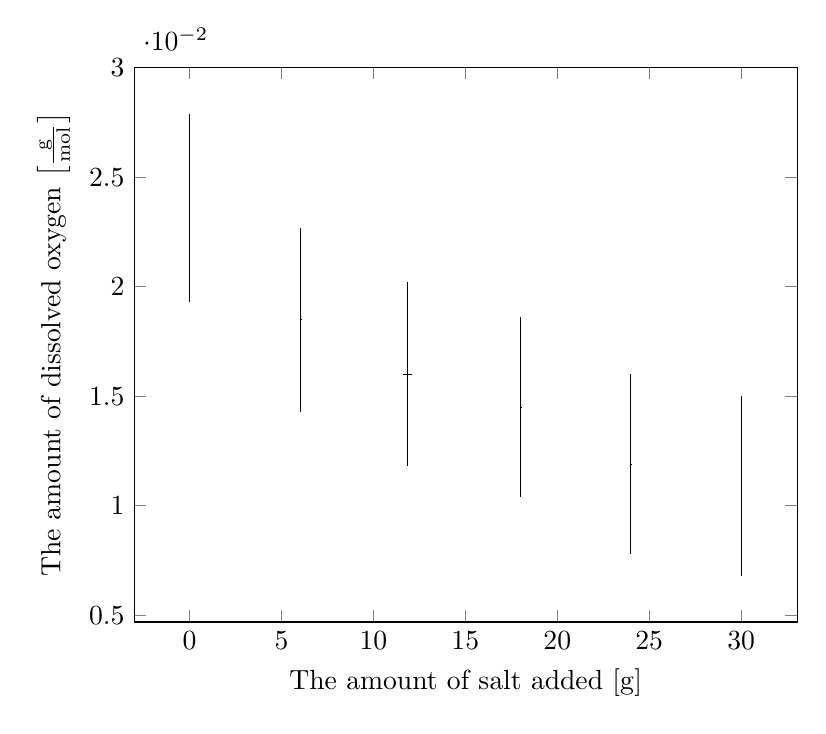
\begin{tikzpicture}
    \begin{axis}[
        ylabel={The amount of dissolved oxygen $\left[ \si{\frac{g}{mol}}
        \right]$},
        xlabel={The amount of salt added $\left[ \si{g} \right]$}
      ]
      \addplot[
        mark=o,
        mark size = 0pt,
        only marks
      ]
        plot [
          error bars/.cd,
          x dir=both,
          x explicit,
          y dir=both,
          y explicit
        ]
        coordinates {
          (0.00, 2.36*0.01) +- (0.00, 0.43*0.01)
          (6.05, 1.85*0.01) +- (0.03, 0.42*0.01)
          (11.87, 1.60*0.01) +- (0.24, 0.42*0.01)
          (18.01, 1.45*0.01) +- (0.03, 0.41*0.01)
          (23.99, 1.19*0.01) +- (0.05, 0.41*0.01)
          (30.01, 1.09*0.01) +- (0.03, 0.41*0.01)
        };
    \end{axis}
  \end{tikzpicture}
  \caption{The graph of the relationship between the mass of salt added and the
  amount of sodium thiosulfate employed.}
  \label{fig:relationship}
\end{figure}

\paragraph*{}
The first fit produced was done using a \textit{python} (Python Software
Foundation) script. This script is given in the appendix. The results are shown
in figure \ref{fig:plot-1}. Note that the domain of the graph is extended.
\begin{figure}[ht]
  \centering
  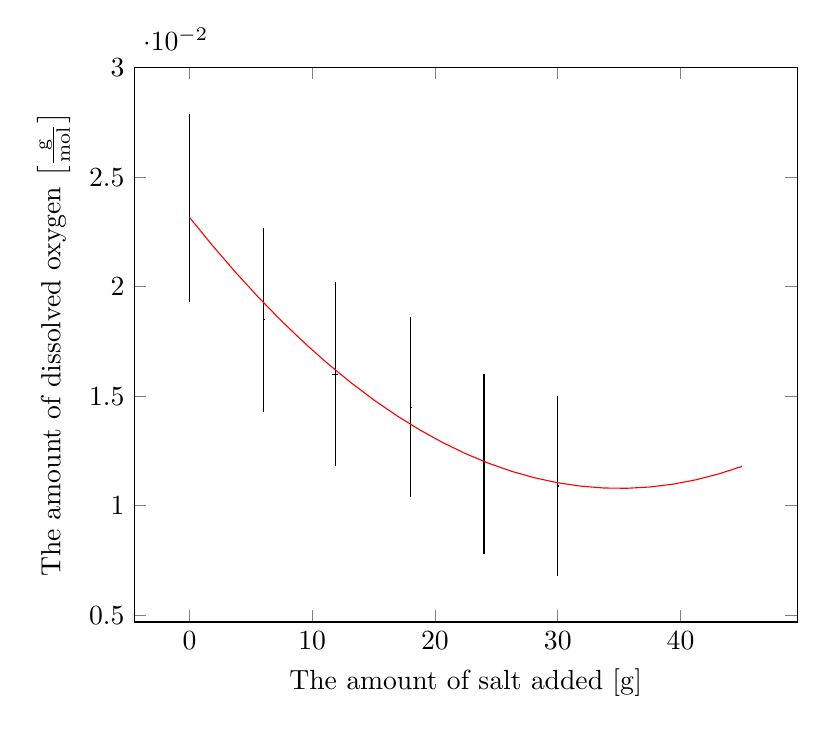
\begin{tikzpicture}
    \begin{axis}[
        ylabel={The amount of dissolved oxygen $\left[ \si{\frac{g}{mol}}
        \right]$},
        xlabel={The amount of salt added $\left[ \si{g} \right]$}
      ]
      \addplot[
        mark=o,
        mark size = 0pt,
        only marks
      ]
        plot [
          error bars/.cd,
          x dir=both,
          x explicit,
          y dir=both,
          y explicit
        ]
        coordinates {
          (0.00, 2.36*0.01) +- (0.00, 0.43*0.01)
          (6.05, 1.85*0.01) +- (0.03, 0.42*0.01)
          (11.87, 1.60*0.01) +- (0.24, 0.42*0.01)
          (18.01, 1.45*0.01) +- (0.03, 0.41*0.01)
          (23.99, 1.19*0.01) +- (0.05, 0.41*0.01)
          (30.01, 1.09*0.01) +- (0.03, 0.41*0.01)
        };
        \addplot[
          color=red,
          domain=0:45
        ]{1.00839942 * 10^(-5) * x^2 - 7.06457161 * 10^(-4) * x + 2.31642928 *
        10^(-2)};
    \end{axis}
  \end{tikzpicture}
  \caption{The graph of the relationship between the mass of salt added and the
  amount of sodium thiosulfate thiosulfate}
  \label{fig:plot-1}
\end{figure}

\paragraph*{}
The fitted function is a quadratic polynomial $a x^2 + bx + c$ with the
coefficients:
\begin{align}
  \label{eqn:coeffs-1}
  a &= 1.00839942 \cdot 10^{-5} \nonumber \\
  b &= -7.06457161 \cdot 10^{-4} \\
  c &= 2.31642928 \cdot 10^{-2} \nonumber
\end{align}

\paragraph*{}
The extended domain shows an issue with this graph - it is impossible for the
amount of dissolved oxygen to increase after it has reached a minimum. The
minimum can be expected to be found at the maximum solubility of $NaCl$ at $t =
20 \si{\degree C}$ in water. This value is $\frac{36 \si{g}}{100 \si{ml}}$
(Rumble, John R). At this point, the graph must remain constant, since the
amount of salt added will not further dissolve. Therefore, the $x$ coordinate
of the minimum of the dissolved oxygen function $\left( -\frac{b}{2a},
\frac{\sqrt{b^2 - 4ac}}{4a} \right)$ is equal to $36 \si{g}$ as well as all of
the values bigger than $36 \si{g}$.

\paragraph*{}
Because $-\frac{b}{2a} = 36$ the following relation can be established:
$$b = -72 a$$

\paragraph*{}
The polynomial function only requires two coefficients now:
$$a x^2 - 72 a x + c$$

The final fit function would therefore be:
$$DO(m_{NaCl})_{t = \si{20 \degree C}} = 
\begin{cases}
  a x^2 - 72 a x + c & m_{NaCl} < 36.0 \si{g} \\
  a \cdot 36.0^2 - 72 a \cdot 36.0 + c & m_{NaCl} \geq 36.0 \si{g} \\
\end{cases}
$$

\paragraph*{}
Using another \textit{python} script (Python Software Foundation), again given
in the appendix, the coefficients $a$ and $c$ have been calculated to be:
\begin{align*}
  a &= 9.63668258 \cdot 10^{-6} \\
  c &= 2.31226620 \cdot 10^{2}
\end{align*}

\paragraph*{}
The plot of the final fit is given in figure \ref{fig:plot-final}.
\begin{figure}[ht]
  \centering
  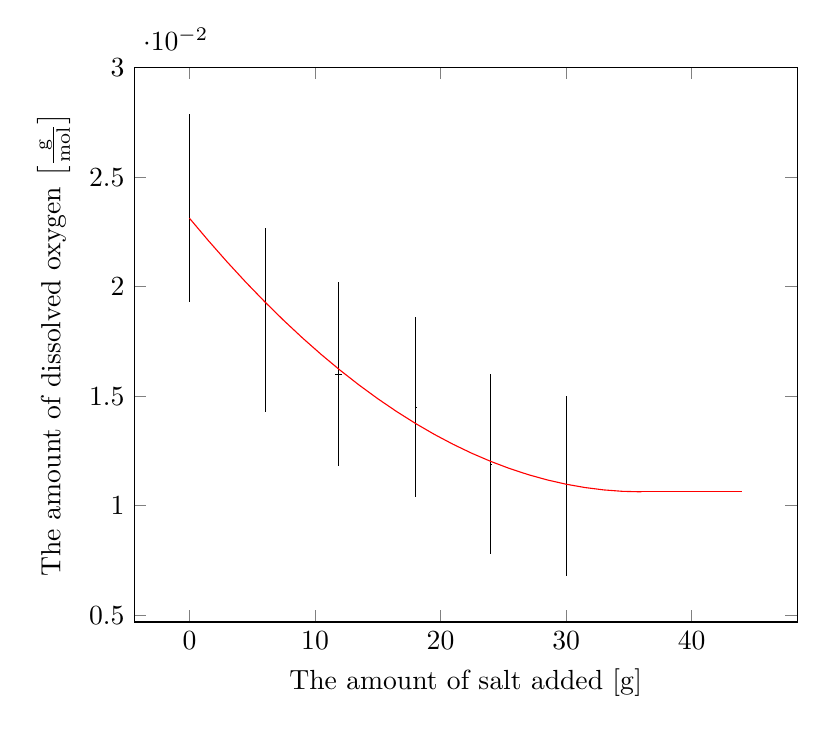
\begin{tikzpicture}
    \begin{axis}[
        ylabel={The amount of dissolved oxygen $\left[ \si{\frac{g}{mol}}
        \right]$},
        xlabel={The amount of salt added $\left[ \si{g} \right]$}
      ]
      \addplot[
        mark=o,
        mark size = 0pt,
        only marks
      ]
        plot [
          error bars/.cd,
          x dir=both,
          x explicit,
          y dir=both,
          y explicit
        ]
        coordinates {
          (0.00, 2.36*0.01) +- (0.00, 0.43*0.01)
          (6.05, 1.85*0.01) +- (0.03, 0.42*0.01)
          (11.87, 1.60*0.01) +- (0.24, 0.42*0.01)
          (18.01, 1.45*0.01) +- (0.03, 0.41*0.01)
          (23.99, 1.19*0.01) +- (0.05, 0.41*0.01)
          (30.01, 1.09*0.01) +- (0.03, 0.41*0.01)
        };
        \addplot[
          color=red,
          domain=0:36
        ]{9.63668258 * 10^(-6) * x^2 - 6.938411458 * 10^(-4) * x + 2.31226620 *
        10^(-2)};
        \addplot[
          color=red,
          domain=36:44
        ]{9.63668258 * 10^(-6) * 36^2 - 6.938411458 * 10^(-4) * 36 + 2.31226620
        * 10^(-2)};
    \end{axis}
  \end{tikzpicture}
  \caption{The graph of the relationship between the mass of salt added and the
  amount of sodium thiosulfate thiosulfate}
  \label{fig:plot-final}
\end{figure}

\subsection{Notes}

\subsubsection{Regarding salt saturation} \label{sec:regarding-salt-saturation}

\paragraph*{}
Note that the coefficients in equation \ref{eqn:coeffs-1} indicate that the
minimum of the dissolved oxygen, according to the formula for the  $x$
coordinate of the minimum of a quadratic function $\left(-\frac{b}{2a} \right)$
is reached at a value of:
\begin{align*}
  -\frac{b}{2a} &= -\frac{-7.06457161 \cdot 10^{-4}}{2 \cdot 1.00839942 \cdot
  10^{-5}} \\
  &= 35.03
\end{align*}

\subsubsection{Errors}

This value indicates that this model predicts that the value of minimal oxygen
saturation, and therefore the maximum amount of $NaCl$ that water can absorb is
a value of $35.03\si{g}$, which indicates an error of only $0.97\si{g}$ or
$2.70\%$. When this is corrected for as explained in the second half of section
\ref{sec:further-calculations}, a more accurate model is achieved.

\paragraph*{}
The uncertainty of the processed data is relatively high. This can be
attributed to the relatively high uncertainty of the titration. Random errors
are obviously at play, at it is unlikely that further measurements will improve
the precision of the experiment.

\paragraph*{}
The information presented in section \ref{sec:regarding-salt-saturation}
implies that the systematic errors were low and that the accuracy of the
experiment was relatively high. Given that the information in section
\ref{sec:regarding-salt-saturation} is completely true, the systematic error
was a measly $2.70\%$. Since the error is minimal, it is possible that this
error stems from random error rather than systematic error.

\section{Conclusion}

\paragraph*{}
The experiment was successful. A minimal systematic error indicates that the
experiment was accurately conducted. For more precise data, however, it would
be preferable that the experiment be conducted with higher volumes of water -
even by a factor of $1 \cdot 10^1$ - $1 \cdot 10^2$. This would minimize the
random error and would improve the overall precision of the results.

\paragraph*{}
The relationship between the amount of $NaCl$ in water and the amount of
dissolved oxygen has been established to be a quadratic one, until the water
becomes saturated with $NaCl$. After this point the added salt plays no effect
on the amount of dissolved oxygen:

$$DO(m_{NaCl})_{t = \si{20 \degree C}} = 
\begin{cases}
  a x^2 + b x + c & m_{NaCl} < 36.0 \si{g} \\
  a \cdot 36.0^2 - 72 a \cdot 36.0 + c & m_{NaCl} \geq 36.0 \si{g} \\
\end{cases}
$$

\paragraph*{}
Regarding the impact of salt and oxygen on marine life - fish which survive in
saltwater require less oxygen - as per the prediction of this study (``HOW
DISSOLVED OXYGEN AFFECTS FISH BEHAVIOUR'').

\paragraph*{}
Overall, as hypothesized, salt content greatly influences the amount of oxygen
that can be dissolved in a water body at a given time.

\singlespacing
\pagebreak
\pagenumbering{gobble}
\section*{Works Cited}
\begin{hangparas}{.25in}{1}
  \begin{sloppypar}
    ``HOW DISSOLVED OXYGEN AFFECTS FISH BEHAVIOUR''. \textit{Active Angling New
    Zealand}, 2019,
    \url{https://activeanglingnz.com/2017/02/23/the-importance-of-dissolved-oxygen/}.
    Accessed 13 Jan 2019. \\

    Feuersanger, Christian. \textit{The PGFPLOTS Package}. Version 1.3,
    Institut Fur Numerische Simulation Universitat Bonn, 2019. \\

    ``Key Physical Variables In The Ocean: Temperature, Salinity, And
    Density''.  \textit{Nature.Com}, 2014,
    \url{https://www.nature.com/scitable/knowledge/library/key-physical-variables-in-the-ocean-temperature-102805293}.
    Accessed 30 Dec 2018. \\

    Merriam Webster. ``Definition Of BIOTOPE''. \textit{Merriam-Webster.Com},
    2018, \url{https://www.merriam-webster.com/dictionary/biotope}. Accessed 30
    Dec 2018. \\

    Python Software Foundation. \textit{Python Language Reference}. Version
    3.6.  \\

    Rumble, John R. CRC \textit{Handbook Of Chemistry And Physics}. 99th ed.,
    CRC Press, 2018. \\

    Senese, Fred. ``General Chemistry Online: FAQ: Solutions: How Can I Predict
    Oxygen Solubility In Water?''. Antoine.Frostburg.Edu, 2015,
    \url{http://antoine.frostburg.edu/chem/senese/101/solutions/faq/predicting-DO.shtml}.
    Accessed 7 Jan 2019. \\

    ``Sodium Iodide''. \textit{Pubchem.Ncbi.Nlm.Nih.Gov}, 2018,
    \url{https://pubchem.ncbi.nlm.nih.gov/compound/sodium_iodide#section=U-S-Exports}.
    Accessed 30 Dec 2018. \\

    ``Sodium Thiosulfate''. \textit{Pubchem.Ncbi.Nlm.Nih.Gov}, 2018,
    \url{https://pubchem.ncbi.nlm.nih.gov/compound/Sodium_thiosulphate#section=GHS-Classification}.
    Accessed 30 Dec 2018. \\

    ``Sulfuric Acid''. \textit{Pubchem.Ncbi.Nlm.Nih.Gov}, 2018,
    \url{https://pubchem.ncbi.nlm.nih.gov/compound/sulfuric_acid#section=Safety-and-Hazards}.
    Accessed 30 Dec 2018. \\

    Utah State University Extension. ``Dissolved Oxygen'',
    \textit{Extension.Usu.Edu}, 2017,
    \url{https://extension.usu.edu/waterquality/learnaboutsurfacewater/propertiesofwater/dissolvedoxygen}.
    Accessed 30 Dec 2018. \\
  \end{sloppypar}
\end{hangparas}

\pagebreak
\section*{Appendix}

\subsection*{First fit script}
\inputminted{python}{../fit1.py}

\subsection*{Second fit script}
\inputminted{python}{../fit2.py}

\end{document}
